\newpage
\begin{song}{title={Piosenka pisana nocą}, music={Coma}}
    \small
    \begin{info}
        \writechord{G6} --- przesuń \writechord{Fmaj7} dwa progi w górę, złap kciukiem bas na 3.\ progu \\
        \writechord{D11/A} --- przesuń \writechord{C/G} dwa progi w górę
    \end{info}
    \begin{multicols}{2}
    \begin{intro}
        \writechord{Fmaj7} \writechord{a} \\
        \writechord{G6} \writechord{D11/A}
    \end{intro}
    \begin{verse}
        ^{Fmaj7} Zapomniałem nakr^{a}ęcić czas \\
        ^{G6} I zapomniałem rozp^{D11/A}ocząć nowy dzień \smallskip \\
        W zagubionej przestrzeni trwam \\
        Cały świat płynie obok gdzieś \medskip \\
        A może ja jestem opowieść \\
        Zmęczonych ust \\
        Znudziłem się Bogu \\
        W połowie, w połowie
    \end{verse}
    \begin{chorus}
        ^{C}Nie ma już nic \\
        ^{e}Nie ma już nic \\
        ^{G6}Nie ma już nic po ta^{D11/A}mtej stronie \smallskip \\
        Nie ma już nic \\
        Nie ma już nic \\
        Nie ma już nic za  ścianą powiek
    \end{chorus}
    \vfill\null\columnbreak{}
    \begin{verse}
        Nie potrafię dokończyć spraw \\
        I nie potrafię wypełnić własnych słów \\
        Jutro zginie ostatni ślad \\
        Zapomnicie że byłem tu \smallskip \\
        A może ja jestem opowieść \\
        Zmęczonych ust \\
        Znudziłem się Bogu \\
        W połowie, w połowie
    \end{verse}
    \begin{chorus}
        Nie ma już nic\ldots
    \end{chorus}
    \begin{interlude}
        ^{e}Jeszcze raz ^{D} mógłbym z^{e}mienić ksz^{D}tałt \\
        Rozpiąć skr^{e}zydła i f^{D}runąć, nie zwa^{e}żając na st^{D}rach \\
        ^{e}Jeszcze raz, ^{D} przecież s^{e}posób z^{D}nam \\
        Tylko ^{e}nie mam już ^{D}siły, tylko ^{e}nie wiem ^{D}jak \bigskip \\
        \writechord{Fmaj7} \writechord{a} \\
        \writechord{G6} \writechord{D11/A}
    \end{interlude}
    \begin{chorus}
        Nie ma już nic\ldots
    \end{chorus}
    \end{multicols}
    \begin{center}
        \vfill{}
        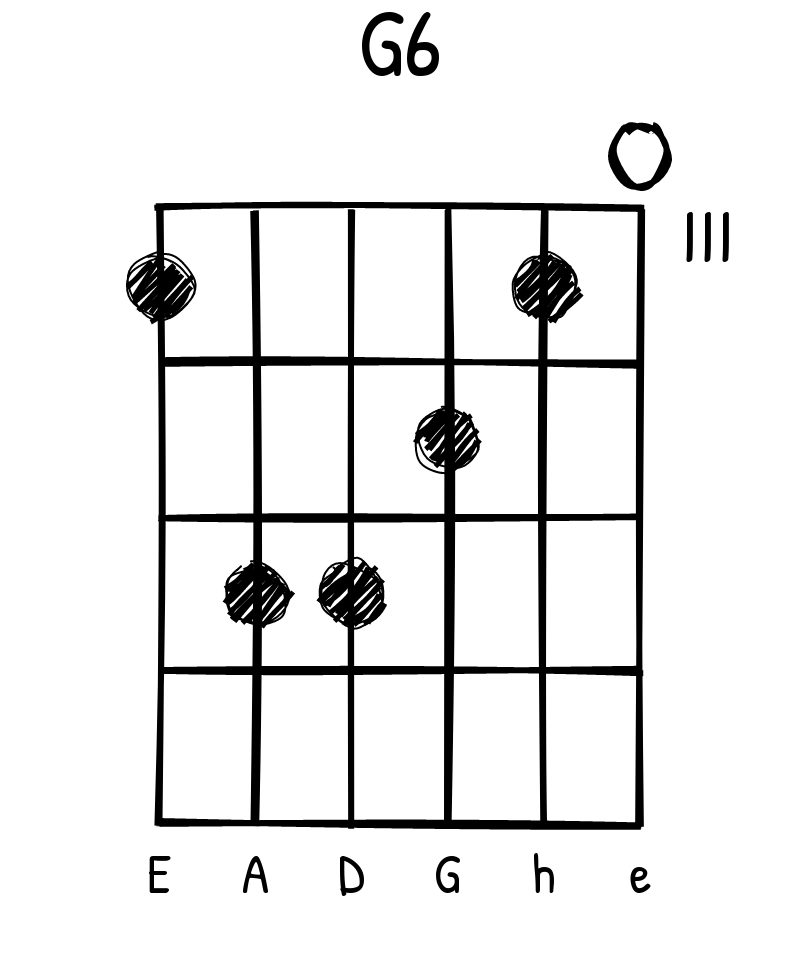
\includegraphics[height=3.5cm]{images/G6.png}
        \hspace{1cm}
        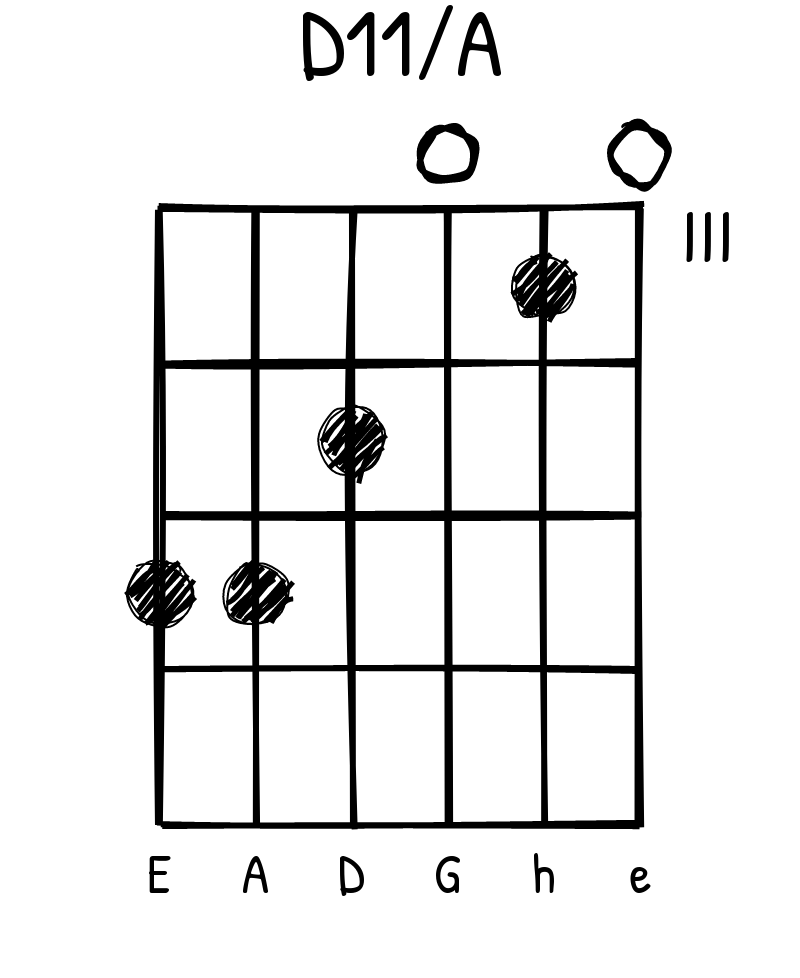
\includegraphics[height=3.5cm]{images/D11A.png}
        \vfill{}
    \end{center}
\end{song}

